\documentclass[a4paper, 11pt]{article}
\usepackage[utf8]{inputenc}
%\usepackage[ansinew]{inputenc}
\usepackage{german}
\usepackage{geometry}
\usepackage{amsmath}
\usepackage{amssymb}
\usepackage{graphicx}
\usepackage{color}
\usepackage{verbatim}
\usepackage{subfig}

\newcommand{\code}[1]{\texttt{#1}}
\newcommand{\codeex}[2][0.98\textwidth]{\vspace*{1ex}\noindent\fbox{\parbox{#1}{\verbatiminput{#2}}}\vspace*{1ex}}
\newcommand{\todo}[1]{\textcolor{red}{\textsc{ToDo:} #1}}
\newcommand{\DerWeg}{\textit{DerWeg }}  % die Leerstelle ist wichtig!
\newcommand{\AnicarViewer}{\textit{AnicarViewer }}  % die Leerstelle ist wichtig!

\geometry{
  body={16cm, 24.7cm},
  left=2.5cm,
  top=2.5cm
}

\title{Überblick über die Hard- und Software im KognitiveAutomobileLabor}
\author{Dr. Martin Lauer, Dipl.-Ing. Bernd Kitt}
\date{11. April 2011}

\begin{document}\sloppypar{
\maketitle

\tableofcontents

\section{Hardware}

\subsection{AniCar}
Bei dem Fahrzeug handelt es sich, von wenigen Komponenten abgesehen, um eine komplette Eigenkonstruktion des Instituts für Mess- und Regelungstechnik. Das Fahrzeug wurde so konzipiert, dass es den Anforderungen des Kognitive Automobile Labors gerecht wird und eine einfache Bedienung ermöglicht. Die Inbetriebnahme der Fahrzeuges erfolgt in drei Schritten:
\begin{itemize}
\item{Spannungsversorgung herstellen (Akkus einschalten und anschließen)}
\item{Komponenten anschließen (Kameras)}
\item{Laptop anschließen (USB, Ethernet)}
\end{itemize}
Sämtliche Anschlüsse am Fahrzeug sowie die Kabel sind beschriftet, sodass eine einfache Verkabelung möglich ist. Ein Vertauschen der Stecker ist nicht möglich.
\begin{figure}[htb]
\centering
\captionsetup[subfloat]{nearskip = -3pt}
\subfloat[Komplettansicht]{\includegraphics[width=75mm]{anicar}\label{fig:anicar}}\quad
\subfloat[Details]{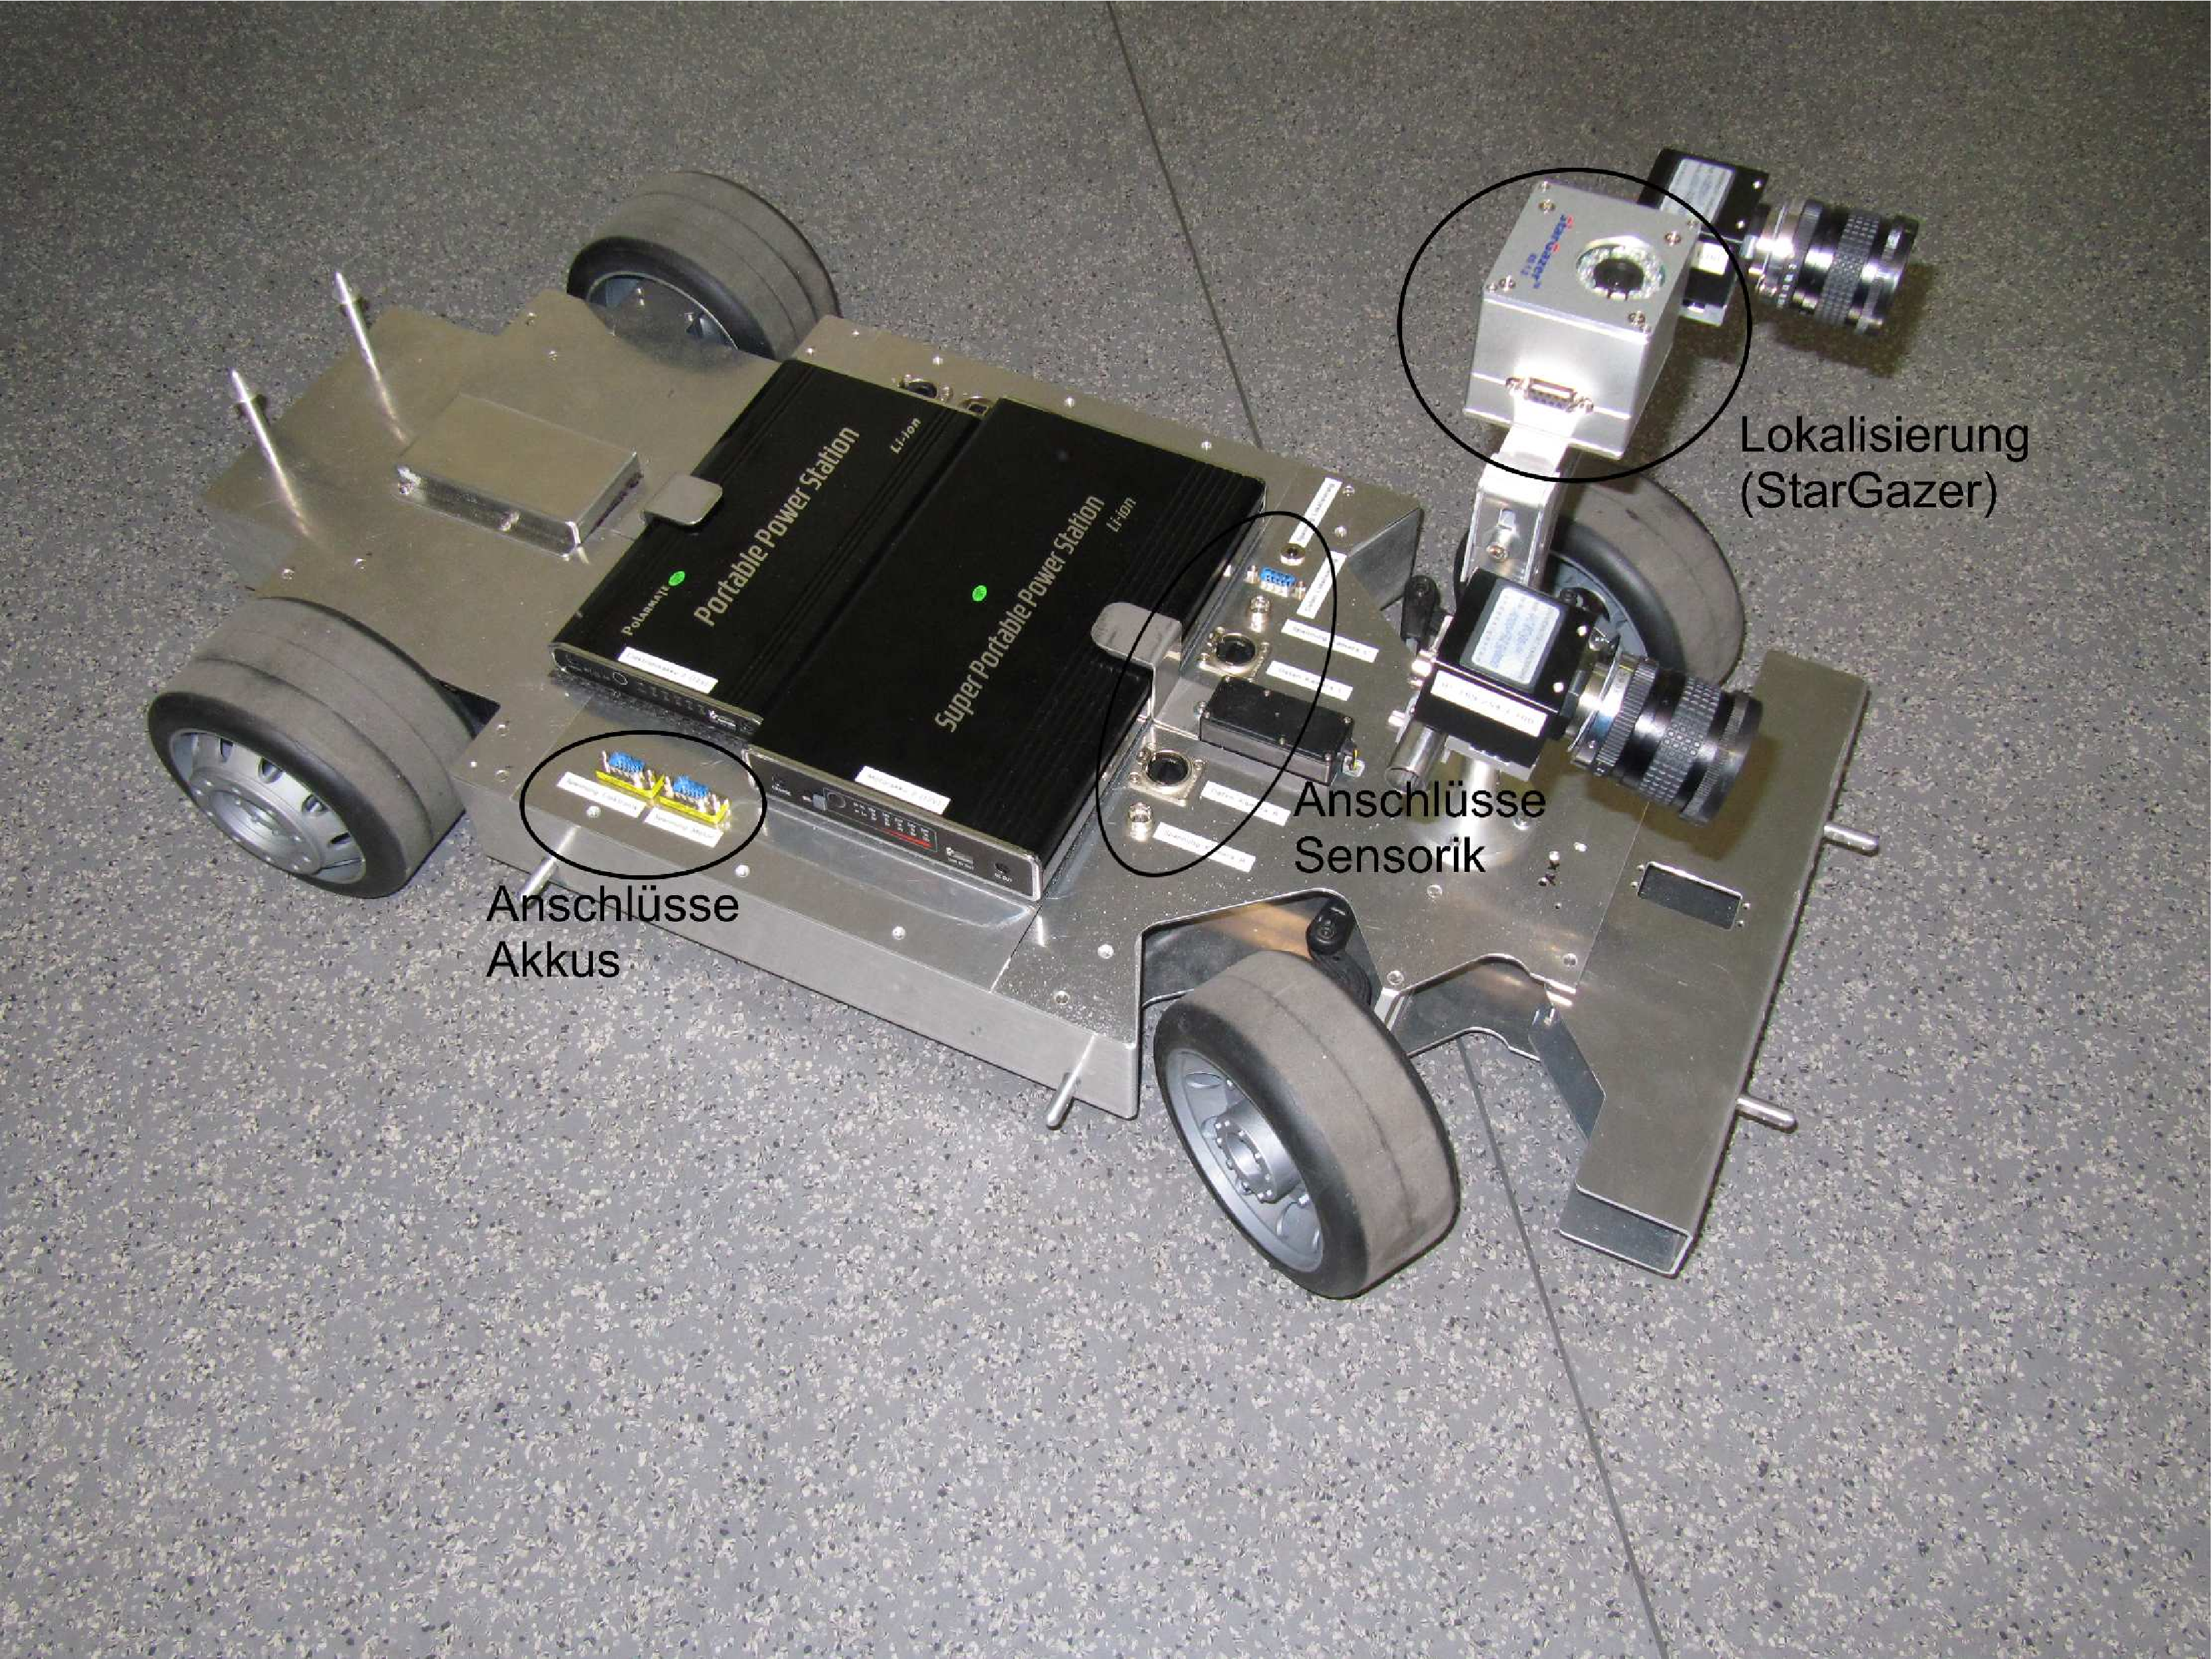
\includegraphics[width=75mm]{anicarSensors}\label{fig:sensors}}
\captionof{figure}[]{AniCar}
\label{fig:anicarImage}
\end{figure}
Das Fahrzeug darf ausschließlich von den Labor-Betreuern geöffnet werden. Das Austauschen der Akkus, darf auch von den Studenten durchgeführt werden.

\subsection{Akkus}
Die Akkus werden durch langes Drücken des Knopfes (Elektronikakku) bzw. mit Hilfe des Schalters (Motorakku) ein- bzw. ausgeschaltet. Die Spannung kann mit Hilfe des Knopfes (lang drücken bis die LED blinkt, dann loslassen) eingestellt werden. Ein kurzes Drücken des Knopfes zeigt den Ladezustand des Akkus an. Der kleinere Akku sollte für die Elektronik, der größere für den Motor verwendet werden. Aufgrund der gleichen Spannung führt eine Verwechslung jedoch nicht zu Beschädigungen.\\
\newline
Hinweise:
\begin{itemize}
\item{Nach Verwendung die Akkus bitte wieder ausschalten.}
\item{\textbf{Die Akkus nur mit 12V betreiben! (Schalter auf "`Lo"').}}
\end{itemize}

% \subsection{Lokalisierung (StarGazer)}
% Der \textit{StarGazer} ist ein Lokalisierungssystem für Indoor-Roboter. Es basiert auf Landmarken die an der Decke montiert sind. Diese werden mit Infrarot-LEDs, die im StarGazer verbaut sind, angestrahlt. Das reflektierte Licht wird mit einer Kamera aufgenommen\footnote{Aufgrund des Infrarotanteils des Sonnenlichtes sind Aussetzer in der Lokalisierung zu erwarten. Aus diesem Grunde werden aktive Landmarken eingesetzt, die selbst Infrarotlicht aussenden. Dies führt zu einer deutlich zuverlässigeren Lokalisierung.}. Basierend auf diesem Bild ist es möglich, die Position und Ausrichtung des StarGazers, d. h. des Fahrzeuges, relativ zur entsprechenden Landmarke zu bestimmen. Die Umrechnung vom "`Landmarkenkoordinatensystem"' ins globale Parcours-Koordinatensystem ist bereits implementiert, sodass sich die gelieferte Pose auf den Parcours bezieht.
\subsection{Lokalisierung}
Die Selbstlokalisierung des Fahrzeugs beruht auf die Landmarken an der Decke und der nach oben gerichteten Kamera auf dem Fahrzeug. Die Landmarken sind mit Infrarot-LEDs ausgestattet, die eine Landmarken-ID sowie ein lokales Koordinatensystem der Landmarke definieren. Die nach oben gerichtete Kamera detektiert die Landmarken und berechnet aus den erkannten Landmarken die Fahrzeugposition sowie die Fahrzeugorientierung.

\subsection{Kameras}
Bei den Kameras handelt es sich um Farbkameras mit Gigabit-Ethernet Anschluss. Dieser erlaubt, je nach verwendeter Auflösung, Bildwiederholraten von bis zu 200 Frames pro Sekunde.

\section{Fahrzeugsteuerprogramm \DerWeg}

Im Fahrzeugsteuerprogramm \DerWeg wird das Verhalten des Fahrzeugs festgelegt. Es wird auf dem AniCar-Rechner gestartet. Es liest die Sensoren des Fahrzeugs (Kamera, Lokalisierungssystem, Odometrie) aus, steuert den Fahr- und den Lenkmotor an, analysiert die Kamerabilder, berechnet daraus ein adäquates Verhalten und regelt Geschwindigkeit und Lenkwinkel. Die Kommunikation mit den Sensoren sowie die Ansteuerung der Motoren sind bereits im Rahmenprogramm, das im Praktikum zur Verfügung gestellt wird, enthalten während die Bildanalyse, Verhaltensgenerierung und Regelung im Praktikum ergänzt werden müssen. Lediglich einige Demoanwendung wurden bisher implementiert (siehe Abschnitt \ref{sec:modules}).

\subsection{Softwarestruktur}

Das Programm \DerWeg ist modular aufgebaut und folgt einer sogenannten \textit{Blackboard-Architektur}. Das bedeutet, innerhalb der Software gibt es mehrere Module, die voneinander unabhängig sind. Alle Module haben Zugriff auf ein Blackboard, von dem sie Informationen über den Status des Fahrzeugs und Sensorinformationen lesen und schreiben können. Der Datenaustausch zwischen den verschiedenen Modulen erfolgt also ausschließlich über das Blackboard. Abbildung \ref{fig:blackboardArchitecture} illustriert diesen Aufbau.

Die einzelnen Module sind eigenständige Threads, d. h. jedes Modul hat eine Funktion \code{execute()}, die quasi parallel zu den anderen Modulen ausgeführt wird. Eine zeitliche Synchronisierung der verschiedenen Module ist nicht per se vorgesehen, allerdings verfügt das Blackboard über Mutexe und Konditionalvariablen\footnote{zu deutsch: Sperren und Signale}, die in einem gewissen Rahmen eine Synchronisierung der Module erlauben und den Zugriff auf das Blackboard Thread-sicher (d. h.: konfliktfrei) gestaltet.

\begin{figure}
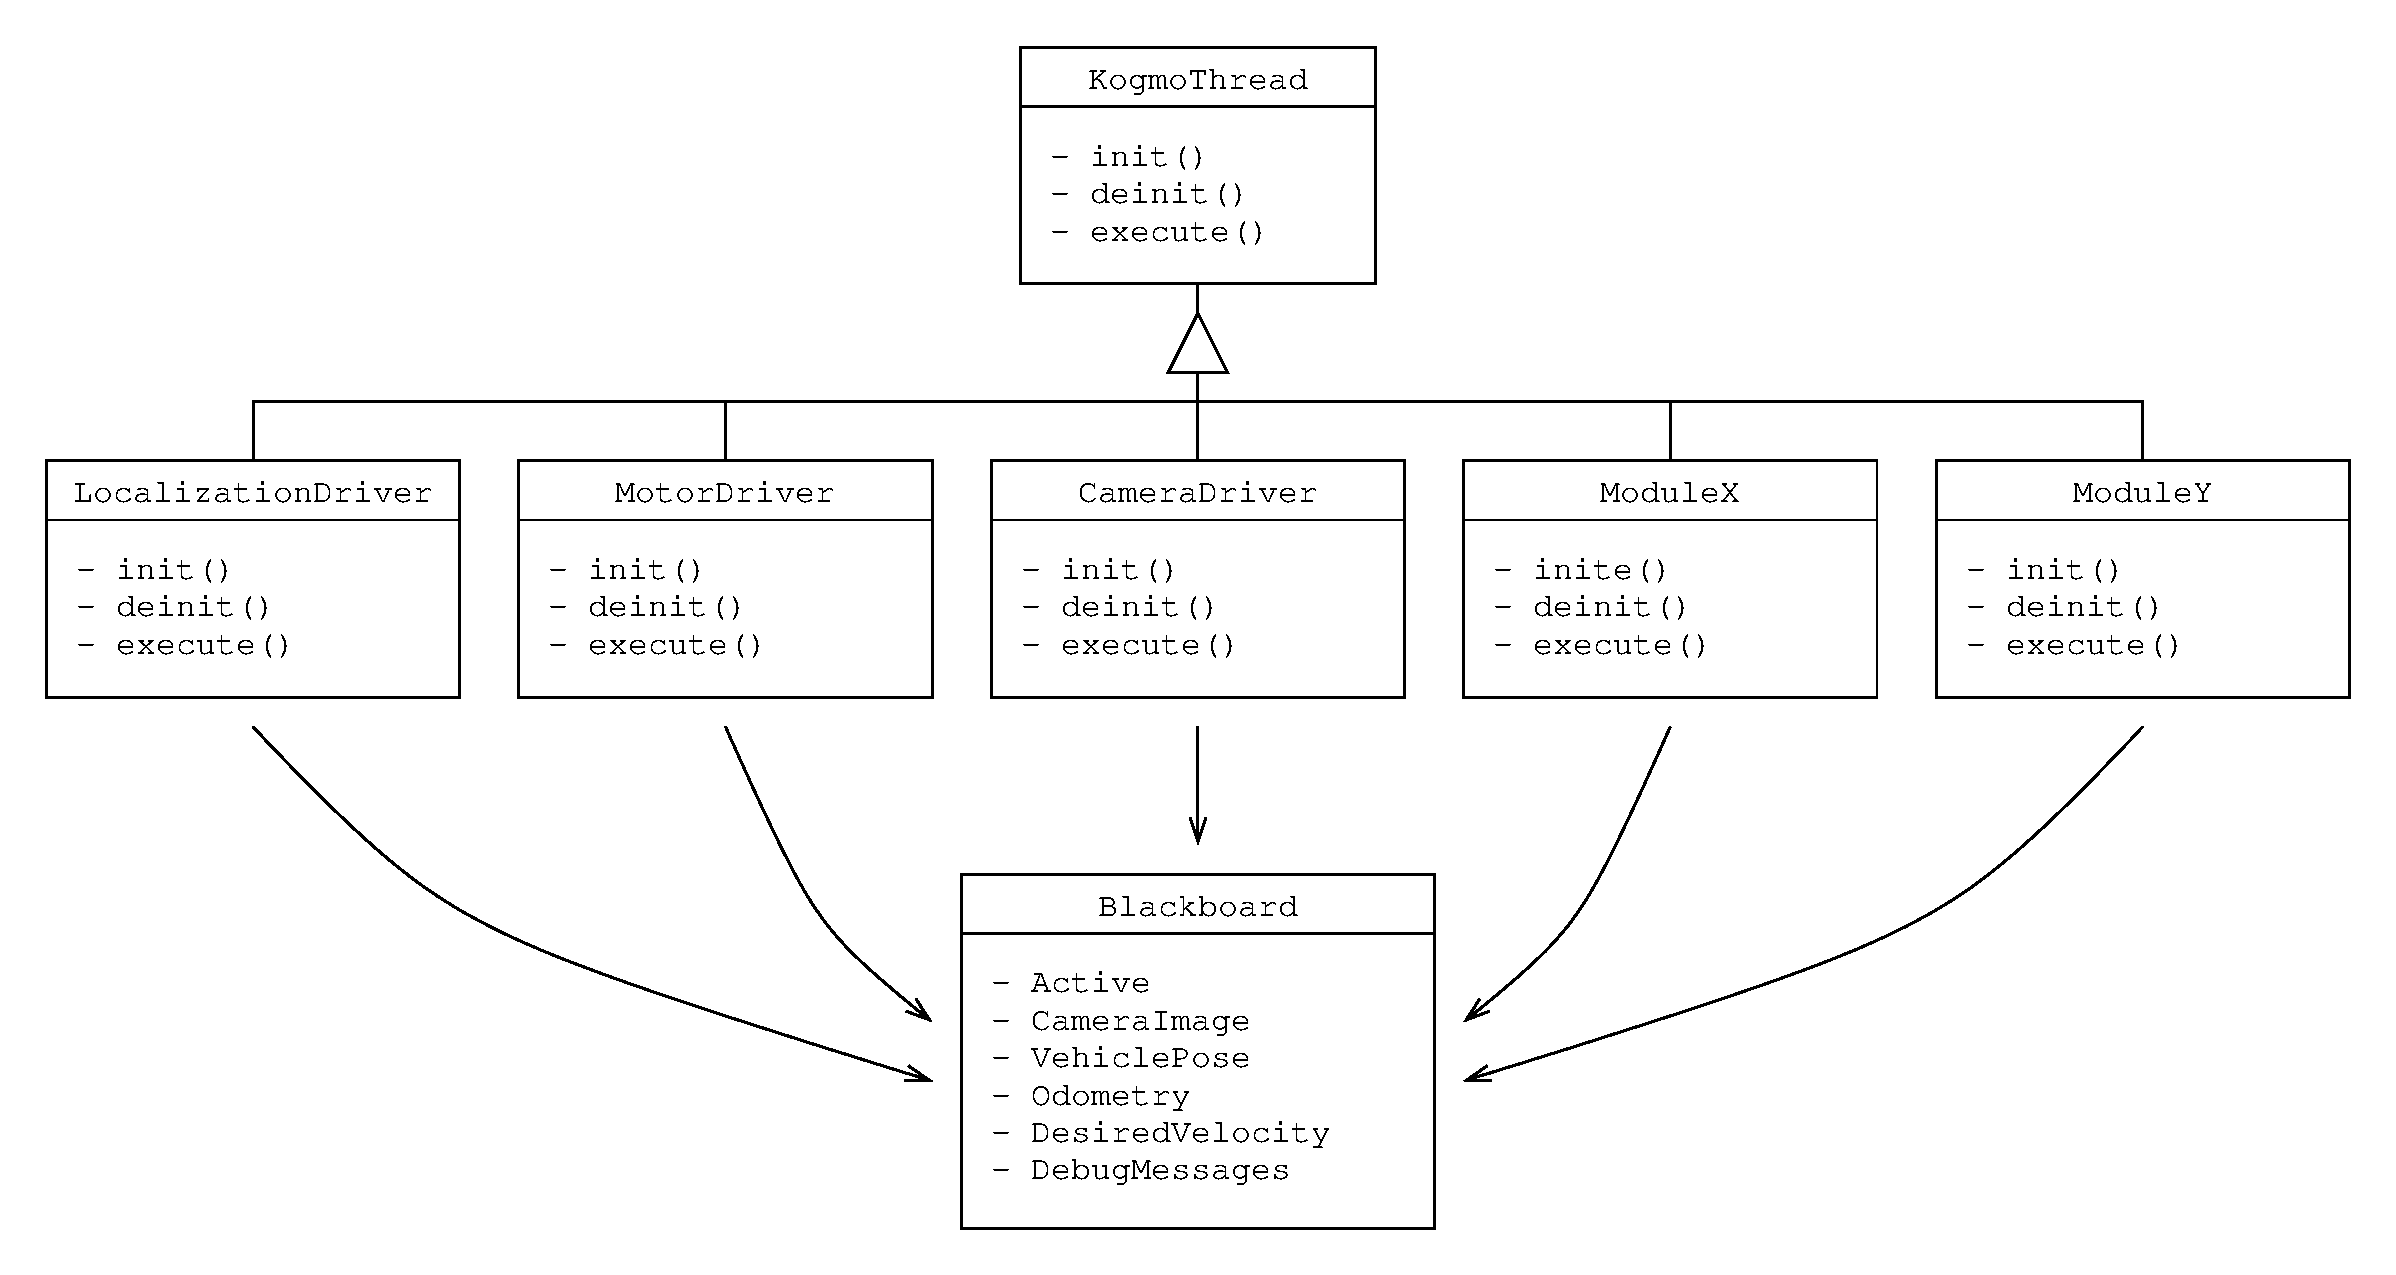
\includegraphics[width=\textwidth]{blackboardArchitecture}
\caption{Schema der Blackboard-Architektur. Alle Module sind eigene Threads, die von der Klasse \code{KogmoThread} abgeleitet sind. Sie besorgen sich alle relevanten Informationen aus dem Blackboard und legen die Ergebnisse ihrer Berechnungen dort wieder ab. Es gibt keine direkte Koppelung verschiedener Module.}
\label{fig:blackboardArchitecture}
\end{figure}

\subsubsection{Das Blackboard}
Das Blackboard ist ein Objekt, auf das alle Module zugreifen können. Das Blackboard enthält im Wesentlichen folgende Informationen:
\begin{itemize}
\item den Status des Fahrzeugs (aktiviert/deaktiviert)
\item Position, Ausrichtung, Geschwindigkeit und Gierrate (Geschwindigkeit und Gierrate berechnet aus den zuletzt gemessenen Fahrzeugpositionen)
\item die Odometrie des Fahrzeugs (Geschwindigkeit gemessen am Rad sowie Lenkwinkel)
\item die Sollgeschwindigkeit und der Soll-Lenkwinkel
\item das aktuelle Kamerabild
\end{itemize}

Der Zugriff auf das Blackboard ist denkbar einfach. Für jede der verfügbaren Informationen gibt es drei Methoden (vgl. Anhang \ref{app:blackboard}):
\begin{itemize}
\item \code{X getX ()} liefert die Information vom Typ X ($X\in \{ \text{Active}, \text{VehiclePose}, \text{Odometry},\linebreak \text{DesiredVelocity}, \text{Image} \}$)
\item \code{void setX (X)} überschreibt die Information im Blackboard
\item \code{bool waitForX (time\_duration)} hält die Ausführung der aufrufenden Funktion an, bis neue Information vom Typ X vorliegt oder bis ein vorgegebenes, maximales Zeitintervall (default: 1s) verstrichen ist. Liefert \textit{true}, wenn neue Information vorliegt und \textit{false}, wenn das maximale Zeitintervall verstrichen ist, ohne, dass neue Information eingetroffen ist.
\end{itemize}

\paragraph{Beispiel}
Möchte man in einer Funktion \code{f()} aus dem Blackboard die aktuelle Position des Fahrzeugs lesen und anschließend eine Sollgeschwindigkeit schreiben, so programmiert man:

\codeex{beispielBlackboard.cpp}


\subsubsection{Die Module}
Die Module im Programm \DerWeg sind alle eigenständige Threads. Sie sind von einer gemeinsamen Elternklasse \code{KogmoThread} abgeleitet und bieten folgende Schnittstelle:
\begin{itemize}
\item Funktion \code{init()} zum Initialisieren des Moduls
\item Funktion \code{deinit()} zum Deinitialisieren des Moduls
\item Funktion \code{execute()}, die die eigentliche Funktionalität des Moduls realisiert und die als eigenständiger Thread gestartet wird
\end{itemize}

Ein Thread arbeitet wie ein eigenständiges Programm innerhalb des Gesamtprogramms. Die Funktion \code{execute()} übernimmt dabei die Rolle, die in einem C++-Programm normalerweise die Funktion \code{main()} übernimmt, d. h. \code{execute()} übernimmt die Ablaufsteuerung. In unserem Falle wird sie in der Regel als eine Endlosschleife ausgelegt sein.

\paragraph{Beispiel}
Die \code{execute()}-Funktion eines Moduls, das immer wieder die aktuelle Fahrzeugposition auf den Bildschirm schreiben soll, könnte folgendermaßen aufgebaut sein:

\codeex{beispielModulEinfach.cpp}

Wie im Beispiel gezeigt ist die \code{execute()}-Funktion als Endlosschleife ausgeführt, die Funktion wird ihre Berechnung also niemals von selbst beenden. Daher ist es wichtig, innerhalb der Endlosschleife eine Möglichkeit zu schaffen, dass die Endlosschleife "`von außen"' unterbrochen wird. Dies erfolgt mit Hilfe der Funktion  \code{boost::this\_thread::interruption\_point()}, die einen sogenannten Cancel-Punkt definiert.

Wie arbeiten Cancel-Punkte? Möchte ein Thread B einen anderen Thread A abbrechen, so sendet er einen sogenannten Cancel-Request, d. h. eine Aufforderung, sich zu beenden. Thread A reagiert zunächst nicht darauf, merkt sich aber den Cancel-Request. Sobald der Thread A auf einen Cancel-Punkt stößt, prüft er, ob ein Cancel-Request vorliegt. Wenn nein, setzt er die Programmausführung fort. Wenn ja, wird die Programmausführung unterbrochen und eine \code{boost::thread\_interrupted}-Exception geworfen. Nun werden alle weiteren Anweisungen im Programm übersprungen, bis eine \code{catch(boost::thread\_interrupted\&)}-Zeile angetroffen wird. Ab dieser Stelle wird die Programmausführung dann fortgesetzt.

Im Beispiel ist innerhalb der Endlosschleife ein Cancel-Punkt definiert. Wird der Thread (hier also die \code{execute()}-Funktion) zum Abbrechen aufgefordert und erreicht das Programm den Cancel-Punkt, so wird die normale Programmausführung unterbrochen, es wird zum Catch-Block gesprungen und unterhalb des Catch-Blocks weitergearbeitet. Da im Beispiel unterhalb des Catch-Blocks kein Code mehr kommt, wird unmittelbar das Ende der Funktion \code{execute()} erreicht und der Thread beendet sich.

Die Funktionen \code{init()} und \code{deinit()} erlauben die Initialisierung von Variablen sowie die Allokierung bzw. Freigabe von Speicherbereichen und Ressourcen, ähnlich einem Konstruktor bzw. Destruktor. Häufig möchte man einem Modul zu Beginn einige Parameterwerte übergeben, um die Arbeitsweise des Moduls beeinflussen zu können. Beispielsweise muss ein Kamera-Treiber wissen, ob er die Kamera im Grauwertmodus oder im Farbmodus starten soll oder ein Bildverarbeitungsalgorithmus benötigt bestimmte Parameter wie z. B. Schwellwerte, die man nicht im Programmcode fest einprogrammieren möchte.

Um dies zu ermöglichen, wird der \code{init()}-Funktion als Argument ein Objekt des Typs \code{ConfigReader} übergeben. Dieses Objekt liest zu Programmstart eine Konfigurationsdatei ein und wertet diese aus. In der Konfigurationsdatei sind die Parameterwerte nach dem Schlüssel-Wert-Prinzip aufgeführt, d. h. jeder Parameter besitzt ein Schlüsselwort, dem ein Wert zugeordnet wird. Möchte man nun den Wert eines Parameters mit Schlüsselwort "`X"' lesen, so kann man den ConfigReader danach fragen mit Hilfe seiner \code{get()}-Funktionen.

\paragraph{Beispiel}
Der folgende Code liest aus dem \code{ConfigReader} die Parameter \textit{GigE::color\_space}, \textit{GigE::gain} und \textit{GigE::image\_size} aus:

\codeex{beispielConfigReaderAnfrage.cpp}

Wie man sieht, nimmt die \code{get()}-Funktion zwei Argumente: das Schlüsselwort des Parameters sowie eine Referenz auf eine Variable, in die die \code{get()}-Funktion den Wert des Parameters schreibt. Die zweite Variable kann vom Typ \code{string, int, unsigned int, float, double} oder \code{bool} sein, je nachdem, welche Art Parameter angefragt werden soll. Außerdem ist es möglich, Arrays von Werten zu erhalten, indem man als zweites Argument eine Variable vom Typ \code{vector$<$int$>$, vector$<$double$>$}, usw. übergibt. Als Rückgabewert liefert die \code{get()}-Funktion entweder \code{true}, wenn der angefragte Schlüssel gefunden wurde, oder \code{false}, wenn der angefragte Schlüssel nicht gefunden wurde. Der Aufbau der Konfigurationsdatei wird näher in Abschnitt \ref{sec:config} beschrieben.


\subsubsection{Modulverwaltung}
Die Modulverwaltung innerhalb der Software folgt einem Plugin-Konzept, die das Hinzufügen neuer Module auf sehr einfache Weise erlaubt. Möchte man ein neues Modul zur Software hinzufügen, so muss man folgendermaßen vorgehen.
\begin{enumerate}
\item Man leitet eine neue Klasse von der Klasse \code{KogmoThread} ab:

\codeex[0.9\textwidth]{beispielModulAbleiten.cpp}

\item Man meldet das neue Modul bei der Modulverwaltung an und gibt ihm einen eindeutigen Namen, unter dem es später ausgewählt werden kann (hier "`MeinNeuesModul"'):

\codeex[0.9\textwidth]{beispielModulAnmelden.cpp}

\item Man übersetzt die Software \DerWeg neu.
\end{enumerate}
Nach diesen drei Schritten steht das neue Modul in der Software zur Verfügung. Nun muss man es nur noch auswählen, um es nutzen zu können. Dies geschieht über einen zusätzlichen Eintrag in einer Konfigurationsdatei, siehe Abschnitt \ref{sec:config}.


\subsection{Spezielle Klassen und Strukturen}

\subsubsection{Bildverarbeitung}

Zur Verarbeitung von Kamerabildern wird in der Software die Bildklasse \code{ImageBuffer} verwendet, die ein Grauwert- oder Farbbild (bei Stereo-Kamera: beide Bilder) sowie den dazugehörigen Zeitstempel repräsentieren kann. Zur Darstellung des Bildes wird die Bildklasse \texttt{cv::Mat} aus der Softwarebibliothek \textit{opencv} verwendet\footnote{opencv ab Version 2.x}. Ein ausführliches Handbuch zur opencv findet man im Internet unter \texttt{http://opencv.itseez.com/}. Um den Start zu erleichtern folgen hier die wichtigsten Funktionen, um unter opencv auf Bilder zuzugreifen.

Bilder werden in der Klasse \texttt{cv::Mat} gespeichert. Ist \textit{im} ein solches Objekt, dann liefert:
\begin{itemize}
\item \texttt{im.cols} die Breite des Bildes
\item \texttt{im.rows} die Höhe des Bildes
\item \texttt{im.type()} den Bildtyp. Für uns zunächst relevant sind nur zwei Typen:
\begin{itemize}
\item \texttt{CV\_8UC1} Grauwertbild mit 256 Graustufen
\item \texttt{CV\_8UC3} Farbbild mit $256^3$ Farbstufen
\end{itemize}
\item mit der Methode \texttt{at} kann man auf einzelne Pixel zugreifen
\begin{itemize}
\item für Grauwertbilder liefert \texttt{im.at<uchar>(v,u)} den Grauwert des Pixels in der $v$-ten Zeile und $u$-ten Spalte
\item für Farbbilder liefert \texttt{im.at<cv::Vec3b>(v,u)} den Farbwert des Pixels in der $v$-ten Zeile und $u$-ten Spalte. Farbwerte werden im RGB-Farbraum repräsentiert. \textbf{Achtung:} die Anordnung des R-, G- und B-Farbwertes in der opencv ist in umgekehrter Reihenfolge: zuerst der B-Wert, dann der G-Wert und dann der R-Wert, daher wird das Farbmodell auch als \textit{BGR} bezeichnet. Auf die einzelnen Werte greift man mit dem eckige-Klammern-Operator zu: \texttt{im.at<cv::Vec3b>(v,u)[0]} liefert den B-Wert, \texttt{im.at<cv::Vec3b>(v,u)[1]} den G-Wert und \texttt{im.at<cv::Vec3b>(v,u)[2]} den R-Wert.
\end{itemize}
\end{itemize}

% \subsubsection{Gegebene Funktionen}
% \label{sec:gegebene_funktionen}
% 
% Neben den allgemeinen Bildverarbeitungsfunktionen, die durch die \textit{OpenCV} bereits abgedeckt werden, steht eine einfache Funktion zur Detektion und Interpretation von Verkehrsschildern zur Verfügung. Diese kann innerhalb des eigenen Projektes verwendet werden, kann aber auch als Ausgangspunkt für eigene Entwicklungen dienen. Zur Verwendung der Funktion innerhalb des eigenen Codes muss die Datei \code{TrafficSignDetector.h} eingebunden werden. Danach kann die Schilderkennung mittels \code{std::vector<TrafficSign> signs = detector.process(Image);} aufgerufen werden. In dem \code{struct} \textit{signs} stehen alle im Bild detektierten Schilder inklusive deren Bedeutung (z.B. Einfahrt verboten, links abbiegen, etc.). Weiterhin steht jeweils noch der Mittelpunkt sowie die Größe der gefundenen Schilder zur Verfügung.

\subsubsection{Stereo-Bildverarbeitung}
\label{sec:stereo}

Um aus einem Kamerabildpaar des Stereokamerasystems ein Tiefenbild zu erzeugen, d.h. um für jedes Pixel den Abstand von der Kamera zu berechnen, stellen wir einen Disparitätsschätzer zur Verfügung, der diese Aufgabe löst. Das Verfahren nutzt die Grafikkarte des Laptops und arbeitet dadurch sehr schnell. Um es zu nutzen, muss man zunächst ein Objekt der Klasse \texttt{DerWeg::StereoGPU} erzeugen. Der Konstuktor benötigt eine Konfigurationsdatei, die auf den Laptops unter \textit{/home/common/calib.xml} liegt. Anschließend kann der Tiefenschaetzer verwendet werden.

Um für ein Stereobildpaar den Tiefenschätzer zu nutzen, benötigt man zwei Kommandos:
\begin{itemize}
\item \texttt{tiefenschaetzer.runStereoMatching (image\_left, image\_right);} startet die Tiefenschätzung für ein Bildpaar
\item \texttt{tiefenschaetzer.getStereoResults (depth, confidence, disparity, rectified\_left);} wartet ab, bis die Tiefenschätzung fertig gerechnet hat und holt die Ergebnisse ab. \textit{depth} enthält für jedes Pixel die geschätzte Tiefe (Abstand von der Kamera in Metern als float), \textit{confidence} die Sicherheit, mit dem die Tiefe bestimmt werden konnte (0=schlecht bis 255=gut), \textit{disparity} liefert die Disparität und \textit{rectified\_left} das rektifizierte, linke Bild. Wichtig: der Tiefenwert für ein Pixel ist nur dann richtig, wenn die Sicherheit für dieses Pixel groß ist.
\end{itemize}

Zwischen dem Aufruf von \texttt{runStereoMatching} und \texttt{getStereoResults} kann man parallel auf der CPU selbst Berechnungen durchführen, um die Rechenzeit anderweitig zu nutzen, z.B. um eine Segmentierung des Bildes durchzuführen, Ampeln oder Schilder zu erkennen. Der Gesamtablauf sieht also folgendermaßen aus:
  
\codeex[0.9\textwidth]{beispielStereo.cpp}

Ein Codebeispiel zum Arbeiten mit Stereobildern findet man auch in der Datei \textit{Application/ShowStereoCameraImage.cpp}.

\subsubsection{Fahrzeug-Lokalisierung und Fahrzeug-Geschwindigkeit}

Zur Beschreibung der Fahrzeug-Position und Fahrzeug-Geschwindigkeit dienen die Klassen \code{Velocity}, \code{Odometry} und \code{Pose}. Die Sollgeschwindigkeit \code{Velocity} besteht aus zwei Variablen, der Sollgeschwindigkeit in Längsrichtung, angegeben in $\frac{m}{s}$, sowie dem Soll-Lenkwinkel. Diese Geschwindigkeiten werden von der Motoransteuerung verwendet, um den Fahrmotor und den Lenkmotor zu regeln.

Die eingeregelte Geschwindigkeit und der eingestellte Lenkwinkel werden von der Motoransteuerung an \DerWeg zurückgeliefert und stehen als \code{Odometry} zur Verfügung. Allerdings ist zu berücksichtigen, dass die Odometrie die Geschwindigkeit am Radumfang liefert und die tatsächliche Geschwindigkeit des Fahrzeugs durch Schlupf abweichen kann. Ebenso besitzt die Lenkung ein gewisses Lenkspiel von wenigen Grad, so dass der tatsächliche Lenkwinkel vom gemessenen Lenkwinkel abweichen kann.

Als dritte Größe zur Positions- und Geschwindigkeitsbestimmung dient das Lokalisierungssystem, das die Position anhand von Landmarken bestimmt. Die daraus geschätzte Fahrzeugposition und -orientierung steht als \code{Pose}-Klasse zur Verfügung. \code{Pose} besitzt vier Attribute: die gemessene Position des Fahrzeugs, seine Ausrichtung sowie die Geschätzte longitudinale Fahrzeuggeschwindigkeit und den Gierwinkel des Fahrzeugs. Die ersten beiden Größen berücksichtigen die Messungen des Lokalisierungssystems sowie die Odometrie des Fahrzeugs. Die Genauigkeit der Positionsbestimmung liegt in der Regel im Zentimeterbereich, kann allerdings an einige Stellen auf dem Parcours, insbesondere weit entfernt von Landmarken, auch größer sein. Verlässt das Fahrzeug den Parcours, so ist keine Lokalisierung mehr möglich. In diesem Fall wird die Position nur noch anhand der Odometrie fortgeschrieben. Bei hohen Geschwindigkeiten nimmt die Lokalisierungsgüte ab.

Das Referenzkoordinatensystem, in der die Fahrzeugpositionen angegeben werden, ist auf dem Boden der Maschinenhalle eingezeichnet. Die Angaben erfolgen in mm. Die Referenzposition am Fahrzeug, auf die sich die Angaben beziehen, ist die Vorderachsmitte. Winkel werden im Gegenuhrzeigersinn gemessen.

Die Schätzungen der Longitudinalgeschwindigkeit des Fahrzeugs sowie des Gierwinkels erfolgen durch Regression über die gemessenen Positionen der letzten Sekunde. Die Schätzung ist unabhängig von der Odometrie, hinkt der tatsächlichen Geschwindigkeit aber etwas hinterher, was sich insbesondere in Phasen starker Beschleunigung auswirkt.

\subsubsection{Konsolen-Ausgaben}

Normalerweise erfolgen Ausgaben auf der Textkonsole in C++ entweder über die Streams \textit{cout} und \textit{cerr} oder über den C-Befehl \textit{printf}. Allerdings sind diese Programmierkonstrukte nicht Thread-sicher, d. h. ihre Verwendung kann bei Multi-Threading wie im Programm \DerWeg zu unvorhersehbaren Problemen führen, insbesondere zu Deadlocks, d. h. das Programm oder einzelne Module des Programms bleiben scheinbar grundlos stehen und setzen ihre Berechnung nicht fort. Um dies zu verhindern, wurden in \DerWeg die beiden Makros \textit{LOUT} und \textit{EOUT} definiert, die die Funktion von \textit{cout} und \textit{cerr} übernehmen, aber Thread-sicher sind. Die Verwendung von \textit{LOUT} und \textit{EOUT} unterscheiden sich leicht von \textit{cout} und \textit{cerr}. Eine Gegenüberstellung der Thread-sicheren und der unsicheren Variante findet sich in Tabelle \ref{tab:thread_safe_logging}. Zur Nutzung von \textit{LOUT} bzw. \textit{EOUT} muss entweder \texttt{Blackboard.h} oder \texttt{ThreadSafeLogging.h} per \texttt{\#include}-Direktive direkt oder indirekt eingebunden sein, sonst meldet der Compiler beim Übersetzen des Programms einen Fehler.

\begin{table}
\centering
\begin{tabular}{|p{0.45\textwidth}|p{0.45\textwidth}|}
\hline
\multicolumn{1}{|c|}{nicht Thread-sicher} & \multicolumn{1}{c|}{Thread-sicher} \\
\hline
\tt cout $\!<<\!$ \"{}Wert=\"{} $\!<<\!$ i $\!<<\!$ endl; &
\tt LOUT (\"{}Wert=\"{} $\!<<\!$ i $\!<<\!$ endl) \\
\tt cerr $\!<<\!$ \"{}Wert=\"{} $\!<<\!$ i $\!<<\!$ endl; &
\tt EOUT (\"{}Wert=\"{} $\!<<\!$ i $\!<<\!$ endl) \\
\tt printf (\"{}Wert=\%d$\backslash$n\"{}, i); & 
\tt LOUT (\"{}Wert=\"{} $\!<<\!$ i $\!<<\!$ endl) \\
\tt fprintf (stderr, \"{}Wert=\%d$\backslash$n\"{}, i); & 
\tt EOUT (\"{}Wert=\"{} $\!<<\!$ i $\!<<\!$ endl) \\
\hline
\end{tabular}
\caption{Gegenüberstellung von Thread-sicherer und unsicherer Variante zum Ausgeben von Text auf der Textkonsole. Alle Beispiele geben den Text "`Wert="' aus gefolgt von dem Wert der Integer-Variablen \textit{i} und einem abschließenden Zeilenvorschub.}
\label{tab:thread_safe_logging}
\end{table}

\subsection{Benutzerinteraktionen und Visualisierungstools}

Die Software enthält zur Zeit zwei Module, mit denen ein Benutzer mit dem Fahrzeug interagieren kann. Dabei handelt es sich um eine einfache, textbasierte Interaktion über das Konsolenfenster sowie um eine grafische Benutzerschnittstelle.

\subsubsection{Textbasierte Benutzerschnittstelle}
\label{sec:tui}

Das Softwaremodul "`TUI"' bietet eine textbasierte Benutzerschnittstelle. Wird \DerWeg mit diesem Modul gestartet, wird zunächst auf der Konsole ein Hilfetext ausgegeben, der die wesentlichen Kommandos beschreibt, die durch Drücken bestimmter Tasten ausgeführt werden. Diese sind:
\begin{description}
\item[q] (quit) beendet die Programmausführung
\item[g] (go) aktiviert das Fahrzeug. Bei Programmstart ist das Fahrzeug deaktiviert, d. h. Fahrtkommandos werden nicht ausgeführt.
\item[blank] (stop) stoppt und deaktiviert das Fahrzeug
\item[s] (status) zeigt Position und Geschwindigkeit des Fahrzeugs an
\item[c] (configuration) zeigt die geladenen Softwaremodule an
\item[h] (help) zeigt einen Hilfetext an
\item[x,y,+,-] unter bestimmten Umständen können diese Tasten genutzt werden, um das Fahrzeug manuell zu steuern. Dies funktioniert nur dann, wenn keine anderen Module die Sollgeschwindigkeit beeinflussen.
\end{description}

\subsubsection{Grafische Benutzerschnittstelle}
\label{sec:gui}

Neben der textbasierten Benutzerschnittstelle auf dem AniCar-Steuerrechner bietet die Software eine grafische Benutzerschnittstelle namens \AnicarViewer. \AnicarViewer ist ein eigenständiges Programm, das über eine Netzwerkverbindung mit dem Programm \DerWeg kommuniziert. Das ermöglicht, dass \AnicarViewer auf einem anderen Rechner gestartet werden kann als \DerWeg. Beispielsweise wird \DerWeg auf dem AniCar-Steuerrechner gestartet, während \AnicarViewer auf einem Standrechner im Rechnerpoolraum läuft, sofern beide Rechner über eine Netzwerkverbindung (z. B. WLAN) miteinander kommunizieren können. Eine solche Konstellation ermöglicht, dass das Fahrzeug kontrolliert werden kann, ohne dem Fahrzeug hinterherlaufen zu müssen. Andererseits kann das WLAN kurzzeitig für einige Sekunden ausfallen und somit ist das Fahrzeug für diesen Zeitraum nicht mehr remote kontrollierbar.

Die GUI wird gestartet mit dem Aufruf von \texttt{AnicarViewer Hostname}, wobei \texttt{Hostname} die IP-Adresse des Rechners ist, auf dem \DerWeg läuft. Hier sind auch die Bezeichnungen \textit{localhost} und \textit{anicar} möglich. Anschließend erscheint das in Abbildung \ref{fig:AnicarViewerSnapshot} darstellte Fenster.

\begin{figure}
\centering
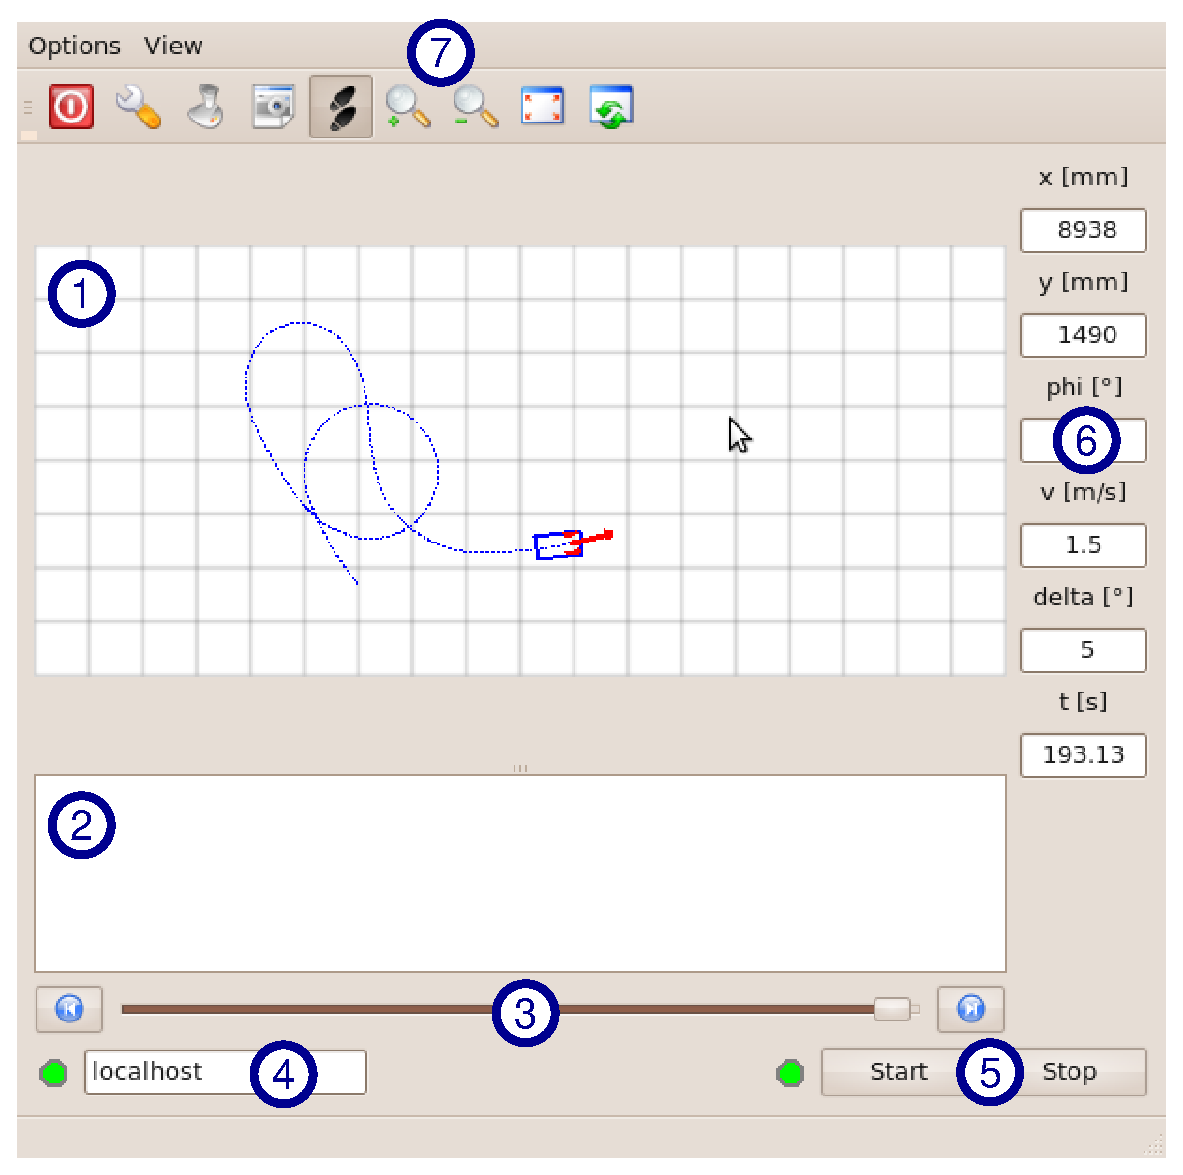
\includegraphics[width=0.8\textwidth]{anicarviewer}
\caption{Ein Bildschirmfoto der grafischen Benutzerschnittstelle \textit{AnicarViewer}. Die Erklärung der einzelnen Bereiche (1)-(7) erfolgt im Text.}
\label{fig:AnicarViewerSnapshot}
\end{figure}

Bereich (1) zeigt eine stilisierte Aufsicht auf den Parcours. Dargestellt wird die momentane Position des Fahrzeugs (blaues Rechteck), der momentane Lenkwinkel (rote Striche), die gegenwärtige Geschwindigkeit (roter Pfeil) sowie ggf. die bisherige Trajektorie (blau gepunktete Linie). Mit den Lupensymbolen (7) kann in die Szene hinein- und herausgezoomt werden, mit den rechts daneben befindlichen Schaltflächen kann die Orientierung der Aufsicht um $90^\circ$ gedreht werden. Die Schaltfläche, die mit den Fußspuren gekennzeichnet ist, schaltet die Darstellung der bisherigen Trajektorie ein bzw. aus. Der in (1) dargestellte, karierte Hintergrund stellt ein regelmäßiges Raster mit Ein-Meter-Abständen dar.

In Bereich (2) werden textuelle Nachrichten dargestellt, die aus dem Programm \DerWeg übertragen wurden. Die Nachrichten stammen aus dem Blackboard und können mit der Methode \code{addMessage()} in das Blackboard geschrieben werden. Die Übermittlung der Nachrichten an \AnicarViewer erfolgt dann automatisch. Die Nachrichten können genutzt werden, um Kontroll- und Debug-Nachrichten zu generieren und somit die Arbeitsweise von \DerWeg während der Laufzeit zu überwachen.

Ähnlich wie die Nachrichten erlaubt \AnicarViewer auch das Einzeichnen einfacher geometrischer Figuren aus \DerWeg in die Aufsicht (1). Hierzu dient die Blackboard-Methode \code{addPlotCommand()}. Die Zeichenkommandos setzen sich aus einem Schlüsselwort und einer variablen Anzahl Argumente zusammen, jeweils durch ein Leerzeichen getrennt. Mehrere Zeichenkommandos können hintereinander geschrieben werden. Der String \texttt{\"{}thick yellow line 1000 2000 4000 2000 5000 3000 green dot 0 0\"{}} beispielsweise zeichnet einen dicken gelben Linienzug mit den Eckpunkten $(1000, 2000)$, $(4000,2000)$ und $(5000,3000)$ und einen grünen Punkt an der Koordinate $(0,0)$. Eine Liste aller Zeichenkommandos ist in Tabelle \ref{tab:plotcmd} aufgeführt.

\begin{table}
\centering
\begin{tabular}{|p{7cm}|p{8cm}|}
\hline
Kommando & Bedeutung \\
\hline
thick & alles dick zeichnen \\
thin & alles dünn zeichnen \\
\hline
solid & mit durchgezogenen Linien zeichnen \\
dashed & mit gestrichelten Linien zeichnen \\
dotted & mit gepunkteten Linien zeichnen \\
\hline
black, white, lightGray, gray, darkGray, red, darkRed, green, darkGreen, blue, darkBlue, yellow, darkYellow, cyan, darkCyan, magenta, darkMagenta & die jeweilige Farbe auswählen \\
\hline
dot $x_1\;y_1\;x_2\;y_2\;\dots$ & Punkte zeichnen an den Koordinaten $(x_1,y_1)$, $(x_2,y_2)$ usw. \\
cross $x_1\;y_1\;x_2\;y_2\;\dots$ & Andreaskreuze zeichnen an den Koordinaten $(x_1,y_1)$, $(x_2,y_2)$ usw. \\
plus $x_1\;y_1\;x_2\;y_2\;\dots$ & Pluszeichen zeichnen an den Koordinaten $(x_1,y_1)$, $(x_2,y_2)$ usw. \\
line $x_1\;y_1\;x_2\;y_2\;x_3\;y_3\dots$ & Linienzug mit den angegebenen Eckpunkten zeichnen \\
arrow $x_1\;y_1\;x_2\;y_2$ & Pfeil von $(x_1,y_1)$ nach $(x_2,y_2)$ zeichnen \\
\hline
\end{tabular}
\caption{Liste aller Zeichenkommandos}
\label{tab:plotcmd}
\end{table}

Der Schieberegler (3) erlaubt das Betrachten der Historie. Die Strecke des Schiebereglers kann als Zeitachse interpretiert werden, wobei der Startzeitpunkt links und der momentane Zeitpunkt rechts liegt. Für alle Zeitpunkte dazwischen speichert \AnicarViewer die Fahrzeugposition und die Nachrichten. Durch Verschieben des Schiebereglers kann man in die Vergangenheit gehen und sich frühere Situationen anschauen. Es ist auch möglich, das Verhalten des Fahrzeugs Schritt für Schritt nachzuvollziehen. Mit Hilfe der Taste "`n"' (next) bewegt man sich einen Zeitschritt weiter, mit "`p"' (previous) einen Zeitschritt zurück.

In (4) wird angezeigt, mit welchem Computer \AnicarViewer eine Verbindung aufbaut. Kann eine Verbindung hergestellt werden (Rechner existiert, Verbindung kann hergestellt werden, \DerWeg wurde gestartet), ist der danebenliegende Punkt grün, ansonsten rot. Mit Hilfe der Schaltflächen in (5) wird das Fahrzeug gestartet und gestoppt (entsprechend den Tasten "`g"' und "'\!$<$\!blank\!$>$\!"' in der TUI). Der grüne bzw. rote Punkt zeigt an, ob das Fahrzeug gestartet ist oder nicht.

Die Anzeigeleiste auf der rechten Seite (6) liefert Informationen über die gegenwärtige Fahrzeugposition, Soll-Geschwindigkeit, Soll-Lenkwinkel sowie eine Systemzeit.

\AnicarViewer bietet zudem die Möglichkeit, einen Joystick anzubinden und mit diesem das Fahrzeug zu steuern. Hierzu wird der Joystick an den Rechner angesteckt, auf dem \AnicarViewer läuft und die Schaltfläche mit dem Joystick-Symbol am oberen Rand des Programmfensters (7) eingeschaltet. Die Schaltfläche mit dem Kamerasymbol veranlasst das Programm \DerWeg, ein Kamerabild abzuspeichern, so dass es nach Ende einer Testfahrt angesehen werden kann. Die Schaltfläche mit dem Schraubenschlüssel-Symbol erlaubt die Anzeige sowie die Veränderung der Module, die \DerWeg verwendet.\footnote{Änderungen wirken sich nur auf das gerade gestartete Programm aus, nicht auf die verwendete Konfigurationsdatei.}

Neben der Möglichkeit, das aktuelle Verhalten des Fahrzeugs zu überwachen, bietet \AnicarViewer auch die Möglichkeit, eine Testfahrt im Nachhinein zu analysieren. Dazu schreibt das Programm ein Logfile names \textit{anicarviewer.log}. Dieses enthält alle Informationen, die \AnicarViewer von \DerWeg bekommen hat. Startet man \AnicarViewer mit \texttt{./AnicarViewer -l logfile}, so liest \AnicarViewer die Daten aus dem Logfile ein, anstatt eine Verbindung mit \DerWeg aufzubauen. Anschließend kann man den Ablauf der Versuchsfahrt im \AnicarViewer nochmals verfolgen und interessante Situationen offline analysieren.

\subsection{Verwendung von \DerWeg}

\subsubsection{Erstinstallation}

Zur Erstinstallation der Software öffnet man eine Textkonsole, wechselt in das Verzeichnis \texttt{KognitiveAutomobileLabor/} und ruft das folgende Kommando auf:
\begin{quote}
make install
\end{quote}


\subsubsection{Programmstart}

Das Programm \DerWeg wird aus einer Textkonsole gestartet mit dem Aufruf: \texttt{./DerWeg} bzw. \texttt{./DerWeg Konfigurationsdatei}, wobei \texttt{Konfigurationsdatei} der Name einer Konfigurationsdatei ist, die die Informationen über die zu startenden Softwaremodule sowie weitere Parameter zu den Softwaremodulen enthält. Wird keine Konfigurationsdatei angegeben, wird die Datei \textit{default.cfg} geladen. Der Aufruf von \DerWeg sollte stets aus dem \texttt{bin/}-Verzeichnis heraus erfolgen, um die richtige Konfigurationsdatei zu finden.

Nach dem Programmstart wird das Programm versuchen, die ausgewählten Module zu initialisieren. Gegebenenfalls werden dabei Debug-Ausgaben in die Konsole geschrieben. Nach Initialisierung aller Module wird jedes Modul gestartet (d. h. die \code{execute()}-Funktion jedes Moduls wird als Thread aufgerufen). Ist es nicht gelungen, alle Module zu initialisieren, so bricht \DerWeg mit einer Fehlermeldung ab.

Hinweis: Soll in der Software Stereobildverarbeitung erfolgen, so muss sie mit \textit{optirun} auf dem Laptop gestartet werden. Hierzu startet man am besten optirun einmal mit dem Kommandozeilenbefehl \texttt{optirun bash}. Anschließend kann man ganz normal \DerWeg starten.

\subsubsection{Konfigurationsdatei}
\label{sec:config}

Die Konfigurationsdatei enthält die Beschreibung der zu startenden Module sowie weitere Parameter für einzelne Module. Sie ist nach dem Schlüssel-Wert-Prinzip aufgebaut, d. h. alle Zeilen haben eine der Formen:
\begin{quote}
Schlüsselwort = Wert\\
Schlüsselwort = Wert1 Wert2 Wert3 ...
\end{quote}
Kommentare werden mit dem Gattersymbol (\#) begonnen, d. h. in folgenden beiden Beispielen werden die mit XXX gekennzeichneten Bereiche ignoriert.
\begin{quote}
\# XXX\\
Schlüsselwort = Wert \# XXX
\end{quote}

Um die Bezeichnung von Schlüsselwörtern konfliktfrei gestalten zu können, gibt es die Möglichkeit, Abschnitte unter eine Überschrift zu setzen, in dem man die Überschrift in eckigen Klammern setzt, z. B.
\begin{quote}
\mbox{}Schlüsselwort1 = Wert1 \\
\mbox{}[Überschrift1] \\
\mbox{}Schlüsselwort2 = Wert2 \\
\mbox{}Schlüsselwort3 = Wert3 \\
\mbox{}[Überschrift2] \\
\mbox{}Schlüsselwort4 = Wert4
\end{quote}
In diesem Fall steht \textit{Schlüsselwort1} unter keiner Überschrift, \textit{Schlüsselwort2} und \textit{Schlüsselwort3} unter der Überschrift \textit{Überschrift1} und \textit{Schlüsselwort4} unter der Überschrift \textit{Überschrift2}. Beim Einlesen setzt der \code{ConfigReader} die Überschrift jeweils vor das Schlüsselwort und trennt beide mit dem doppelten Doppelpunkt \texttt{::} voneinander. Im oberen Beispiel lauten also die vollständigen Schlüsselworte \textit{Schlüsselwort1}, \textit{Überschrift1::Schlüsselwort2}, \textit{Überschrift1::Schlüsselwort3} und \textit{Überschrift2::Schlüsselwort4}.

Mit dem +-Zeichen lassen sich weitere Konfigurationsdateien rekursiv einbinden, z. B. bindet folgende Zeile die Konfigurationsdatei \textit{landmarks.cfg} ein:
\begin{quote}
+ landmarks.cfg
\end{quote}

Um konfliktfreie, gut verständliche Konfigurationsdateien zu erhalten, sollten folgende Konventionen eingehalten werden.
\begin{itemize}
\item das Schlüsselwort \textit{Modules} (ohne Überschrift) ist reserviert für die Liste zu startender Module
\item Parameter, die für ein Modul XXX relevant sind, sollten unter der gleichnamigen Überschrift [XXX] stehen
\item Parameter, die zum selben Modul gehören, sollten räumlich beieinander stehen
\item die Parameter sollten selbsterklärende Namen besitzen und gegebenenfalls durch Kommentare erklärt werden.
\end{itemize}

Die Datei \textit{default.cfg} enthält als Beispiel bereits eine auf dem Fahrzeug lauffähige Konfiguration.

\subsubsection{Verfügbare Module}
\label{sec:modules}

In der Basisausstattung der Software sind bereits einige Module vorimplementiert, die Basisaufgaben wie die Ansteuerung von Kamera und Motor beinhalten, aber auch Beispiele für Bildverarbeitung und Fahrzeugregelung. Die Basismodule sind in Tabelle \ref{tab:modules} aufgezählt.

\begin{table}
\centering
\begin{tabular}{p{0.24\textwidth}p{0.7\textwidth}}
\hline
Name & Funktionalität \\
\hline\hline
\multicolumn{2}{|c|}{\textsc{Lokalisierungsmodule:}} \\
\hline
TopGigE & \raggedright Kameratreiber für die Lokalisierungskamera. Wird für die Lokalisierung zwingend benötigt \tabularnewline
CameraLocalization & \raggedright Lokalisierung anhand von Landmarken. Benötigt zusätzlich das Modul TopGigE \tabularnewline
%StarGazerGyro & \raggedright Lokalisierung anhand von Landmarken und Gyroskop. Arbeitet nur auf AniCar bei eingeschaltetem StarGazer und angebundener Inertialmesseinheit \tabularnewline
%StarGazerOnly & \raggedright Lokalisierung anhand von Landmarken. Arbeitet nur auf AniCar bei eingeschaltetem StarGazer \tabularnewline
DeadReckoning & \raggedright Lokalisierung mittels DeadReckoning, d. h. durch Integration der Odometrie (nur zum Testen). \tabularnewline
ShowLocalization & \raggedright zeigt den gefahrenen Weg auf dem Bildschirm grafisch an \tabularnewline
\hline
\multicolumn{2}{|c|}{\textsc{Module zu Kamera \& Bildern:}} \\
\hline
%GigE & \raggedright Monoskopischer Kameratreiber. Besitzt Möglichkeiten zur Wahl von Bildausschnitt, Weißabgleich und Auto-Exposure \tabularnewline
StereoGigE & \raggedright Kameratreiber für das Stereokamerasystem. Ansonsten wie GigE \tabularnewline
ImagesFromFile & \raggedright lädt gespeicherte Bilder von Festplatte. Verzeichnis und Dateinamen der Bilder können über weitere Parameter in der Konfigurationsdatei bestimmt werden. Kann zum Testen und Debuggen alternativ zu GigE verwendet werden \tabularnewline
SaveCameraImages & \raggedright speichert alle eingehenden Bilder auf der Festplatte. Verzeichnis und Dateinamen können in der Konfigurationsdatei definiert werden. Eignet sich zum Aufnehmen von Bildsequenzen \tabularnewline
ShowCameraImages & \raggedright zeigt circa zwei Bilder bzw. zwei Bildpaare pro Sekunde auf dem Bildschirm an \tabularnewline
ShowStereo \hspace*{2em}\mbox{CameraImages} & \raggedright zeigt circa zwei Stereo-Bildpaare pro Sekunde sowie die geschätzte Stereo-Disparität auf dem Bildschirm an \tabularnewline
\hline
\multicolumn{2}{|c|}{\textsc{Module zur Motoransteuerung:}} \\
\hline
MotorInterface & \raggedright Ansteuerung von Lenk- und Fahrmotor auf dem AniCar. Die Parameter dieses Moduls nicht verändern. \tabularnewline
MotorDummy & \raggedright Eine Pseudo-Motoransteuerung, die nichts anderes tut, als die Sollgeschwindigkeit zu nehmen und als Odometrie wieder ins Blackboard zu schreiben. Alternative zu MotorInterface, wenn man nicht auf dem AniCar arbeitet \tabularnewline
AnicarSimulation & \raggedright Ein Simulator, der das Verhalten des Fahrzeugs simuliert und dabei auch Störeffekte teilweise berücksichtigt. Das Modul ersetzt in der Simulation das Motor-Ansteuerugnsmodul sowie das Lokalisierungsmodul \tabularnewline
\hline
\multicolumn{2}{|c|}{\textsc{Module zur Benutzerschnittstelle:}} \\
\hline
TUI & \raggedright Konsolenbasierte Schnittstelle, siehe Abschnitt \ref{sec:tui}. Sollte immer ausgewählt sein. \tabularnewline
AnicarViewer & \raggedright Grafische Schnittstelle, siehe Abschnitt \ref{sec:gui}. Sollte immer ausgewählt sein. \tabularnewline
\hline
\end{tabular}
\caption{Vorimplementierte Module}
\label{tab:modules}
\end{table} ShowStereoCameraImages

Mit diesen Modulen lassen sich bereits sinnvolle Kombinationen zusammenstellen. Möchte man das Fahrzeug im voll-autonomen Modus fahren lassen, benötigt man zumindest die Module MotorInterface, TopGigE, CameraLocalization, StereoGigE, TUI und AnicarViewer. Möchte man hingegen mit dem Fahrzeug ein manuell (d. h. mit Joystick) gesteuerte Probefahrt machen und dabei die Kamerabilder aufzeichnen, benötigt man die Module MotorInterface, GigE, TUI, AnicarViewer und SaveCameraImages. Hat man anschließend die Testbilder auf einen Standrechner kopiert und möchte nun die Fahrt im Nachhinein nochmals durchspielen, kann man beispielsweise \DerWeg mit den Modulen ImagesFromFile, TUI, AnicarViewer und ShowCameraImages starten. Dadurch kann man beispielsweise einen Bildverarbeitungsalgorithmus so lange testen, bis er fehlerfrei auf den gespeicherten Bildern arbeitet. Zum Testen von Bahnplanungs-, Quer- und Längsregelungsverfahren in der Simulation eignet sich die Kombination der Module TUI, AnicarViewer und AnicarSimulation.

Neben den Basismodulen sind in \DerWeg die Fahrzeugregelungsmodule \textit{StopAtRed}, %\textit{StopAtNoEntry},
\textit{DriveWigglyLines} und \textit{CyclicForwardsBackwards} implementiert, die beispielhaft die Implementierung einer einfachen Verhaltensgenerierung für das Fahrzeug veranschaulichen. Der Quellcode der drei Module befindet sich im Anhang \ref{app:codeexamples} dieses Dokumentes.

StopAtRed führt eine einfache Bildauswertung durch, indem es zählt, welcher Anteil der Pixel im Kamerabild rötlich sind. Ist dieser Anteil höher als ein Schwellwert, dann stoppt das Fahrzeug, ansonsten fährt es langsam geradeaus. Das Modul kombiniert also eine sehr einfache Bildverarbeitung mit der Vorgabe von Geschwindigkeitssollwerten. Die Fahrzeuglokalisierung wird hierbei nicht benötigt. Möchte man sich das Verhalten anschauen, startet man \DerWeg mit der Modulkombination MotorInterface, StereoGigE, TUI, GUI, StopAtRed.

%StopAtNoEntry variiert StopAtRed, indem es den in Abschnitt \ref{sec:gegebene_funktionen} beschriebenen Schildererkenner einbindet, anstatt rote Pixel zu zählen. Ausprobieren kann man dieses Modul mit der Modulkombination MotorInterface, GigE, TUI, GUI, StopAtNoEntry.

Die zweite Demoanwendung implementiert einen sehr einfachen Regler, um der Geraden $y=2000$ zu folgen. Hierbei wird der Lenkwinkel proportional zum Abstand des Fahrzeugs von der Zielgeraden eingestellt. Befindet sich das Fahrzeug mehr als 1,5m von der Geraden entfernt, stoppt das Fahrzeug. Das Modul kombiniert also die Fahrzeuglokalisierung mit einer sehr einfachen Lenkregelung. Kamerabilder werden nicht benötigt, so dass man mit den Modulen MotorInterface, TopGigE, CameraLocalization, TUI, GUI, DriveWigglyLines auskommt.

Die dritte Anwendung CyclicForwardsBackwards arbeitet ohne Bildverarbeitung oder Lokalisierung. Sie steuert den Fahrmotor abwechselnd vor- und rückwärts an und lenkt dabei abwechselnd nach links und rechts, so dass eine sternförmige Bahn abgefahren wird. Das Programm ist ein Beispiel für eine Fahrzeugsteuerung ohne Rückkoppelung (d. h. keine Regelung).

\textit{Bitte beachten:} Die drei Demoanwendungen sind sehr einfach und erkennen nicht, wenn das Fahrzeug den Parcours verlässt. Daher ist es stets erforderlich, jemanden am \AnicarViewer sitzen zu haben, der zur Not auf "`Stop"' drücken kann!


\section{Entwicklungsumgebung}

\subsection{Betriebssystem Linux}

Die Entwicklung der Software erfolgt unter Linux. Das Betriebssystem Linux mag für einige gewöhnungsbedürftig sein, es ist aber auch nicht schwerer zu bedienen als Windows. Wer wie in Windows viel "`Klicken"' will, findet inzwischen auch unter Linux genügend brauchbare Softwaretools. Der Vorteil gegenüber Windows ist jedoch, dass es auch Alternativen zum "`Drag-and-Drop"' und "`Klick"' gibt, die sich häufig nach gewisser Einarbeitszeit als äußerst effizient herausstellen.

Im Unterschied zu Windows spielt unter Linux die Textkonsole (entsprechend dem DOS-Fenster in Windows) eine größere Rolle. Von hier aus kann man durch die Verzeichnisstruktur des Dateisystems browsen und Programme starten (durch Eingeben des Programmnamens, ggf. durch ein vorangesetztes "`./"' ergänzt). Verschiedene Editoren können genutzt werden, um Textdateien zu bearbeiten, u.a. \textit{kate}, \textit{gedit}, \textit{joe} und \textit{vi} (die beiden zuletzt genannten sind etwas schwieriger zu bedienen).

Wir haben auf dem AniCar-Rechner und auf den Standrechnern ein Grundprogramm an Linux-Software installiert, die für die allermeisten Bedürfnisse ausreichen werden. Falls irgendetwas wichtiges fehlt, bitte Bescheid geben, dass wir es nachinstallieren können.

\subsection{Programmiersprache C++}

Die Software \DerWeg ist in der Programmiersprache C++ programmiert. C++ ist eine der am weitesten verbreiteten Programmiersprachen der Welt und eignet sich sehr gut für zeitkritische, systemnahe Anwendungen (im Gegensatz zu Java). Es ist ähnlich zu Java und es sollte für einen Java-Programmierer keine allzu großen Schwierigkeiten bereiten, sich an C++ zu gewöhnen. Ein Tutorial zu C++ von Lutz Frommberger kann unter \texttt{http://www.aussagekraft.de/files/c-intro-handout.pdf} 
bezogen werden.

\subsection{Entwicklungsumgebung}

Unter Linux gibt es eine große Bandbreite an Entwicklungsumgebungen. Wir unterstützen davon allerdings zur Zeit lediglich \textit{Code::Blocks}. Wer bisher mit den Visual-Entwicklungsumgebungen gearbeitet hat, wird bei \textit{Code::Blocks} viel bekanntes wieder finden (siehe Abbildung \ref{fig:codeblockssnapshot}). Die Projektdatei heißt \textit{DerWeg.cbp}.

Wem integrierte Entwicklungsumgebungen zu kompliziert sind, kann die Software natürlich auch in einem gewöhnlichen Texteditor programmieren oder eine andere Entwicklungsumgebung nutzen. Um dies zu ermöglichen, haben wir ein Makefile angelegt, das die \textit{Code::Blocks}-Projektdateien auswertet und die Software übersetzt. Möchte man weitere Dateien zum Projekt hinzufügen, muss man dann die \textit{Code::Blocks}-Projektdateien ergänzen.

\begin{figure}
\centering
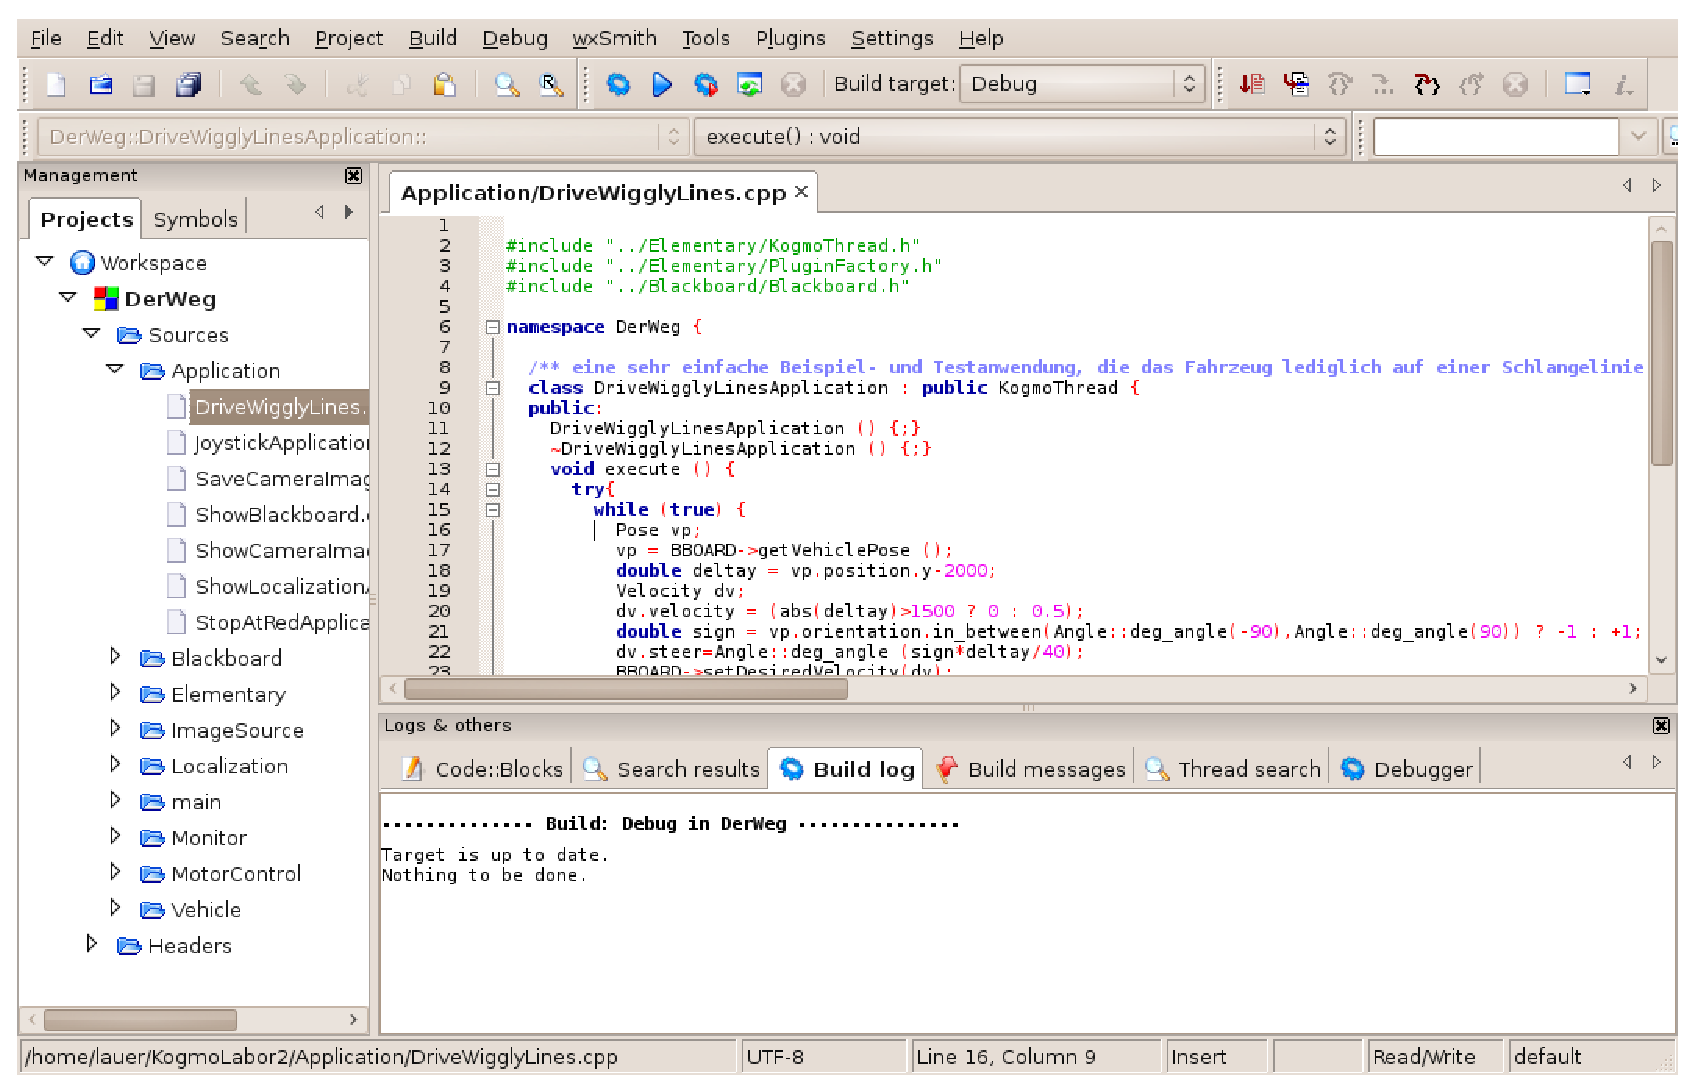
\includegraphics[width=0.8\textwidth]{codeblockssnapshot}
\caption{Ein Bildschirmfoto der Entwicklungsumgebung.}
\label{fig:codeblockssnapshot}
\end{figure}

Einige Hinweise zum Arbeiten mit \textit{Code::Blocks}: 
\begin{itemize}
\item Hinzufügen von Quelldateien: Hat man innerhalb von Code::Blocks eine Quelldatei zum Projekt hinzugefügt, sollte man unbedingt die Projektdatei abspeichern (über Menü$\rightarrow$File$\rightarrow$Save project). Andernfalls wird die neue Datei nicht mitübersetzt.
\item Möchte man die Software auf einem Rechner übersetzen, der keine Cuda-Unterstützung hat, bei dem die Kameratreiber nicht arbeiten oder auf dem eine ältere Version der opencv installiert ist, gibt es die Möglichkeit, durch Auswahl des \textit{Build target} umzuschalten. Die Option \textit{nostereo} verzichtet auf die Stereobildverarbeitungsteile, die Option \textit{nocamera} auf die Kameratreiber einschließlich der Stereobildverarbeitung.
\end{itemize}

\subsection{Software-Upgrades}

Da \DerWeg just-in-time entwickelt wurde, ist nicht auszuschließen, dass wir noch einige Bugfixes und/oder Erweiterungen im Laufe der Zeit nachliefern müssen. Um dies zu erleichtern ist es erforderlich, folgende Konvention einzuhalten: Das Rahmenprogramm von \DerWeg und die zur Basisausstattung gehörenden Module werden ausschließlich von den Labor-Betreuern gewartet. Änderungen dieser Programmteile durch die Labor-Teilnehmer sind nicht zulässig. Hingegen sind die Labor-Teilnehmer verantwortlich für alle Programmteile und Module, die sie zur Basissoftware hinzufügen.

Diese Regelung hört sich zwar wie eine Drangsalierung an, ist aber notwendig, um die Konsistenz der Software zu erhalten. Auch wenn es manchmal vermeintlich die bequemere Lösung zu sein scheint, Teile der Basissoftware zu verändern, ist dies der falsche Weg. Wenn es Bugs in diesen Teilen gibt, bitte den Labor-Betreuern Bescheid sagen. Wenn es fehlende Funktionalität gibt, dann auch erst mal mit den Labor-Betreuern sprechen. Wenn bestehende Demo-Module eine gute Basis für den weiteren Ausbau bieten, dann ist der richtige Weg, diese Module zu kopieren, umzubenennen und nur die kopierte Version zu verändern.

\subsection{Versionshaltung}

Bei einer Softwareentwicklung im Team ist es außerordentlich hilfreich, ein Versionshaltungssystem zu verwenden, das die verschiedenen Dateien der Software verwaltet, ältere Versionen vorhält und die Änderungen meherer Entwickler zusammenführt. Wir stellen dafür für jede Gruppe ein Subversion (SVN)-Repositorium zur Verfügung. Veränderungen an der Basissoftware werden wir ebenfalls über die Repositorien zur Verfügung stellen.

Aus Erfahrung heraus empfehlen wir die Verwendung der SVN-Repositorien dringend. Anfänglich mögen sie einen vermeintlich unnötigen Overhead erzeugen, aber mit der naiven Methode des Dateiaustausches per Email oder USB-Stick wird man schon nach wenigen Wochen sehr unglücklich werden.

\subsection{Programmdokumentation}

Der Programmcode ist dafür vorbereitet, um mit Hilfe von \textit{doxygen} eine HTML-Dokumentation von \DerWeg zu erstellen. Zur Erzeugung der Dokumentation wechselt man in der Konsole in das Projektverzeichnis und ruft \texttt{doxygen} auf. Die HTML-Dokumentation wird dann im Unterverzeichnis \textit{doc/html} erzeugt und kann mit einem beliebigen Browser angesehen werden.

Dieses Dokument befindet sich im Unterverzeichnis \textit{doc/SoftwareDoku} und kann durch Aufruf von \texttt{pdflatex softwaredoku} erzeugt werden.

\appendix

\section{Anhang: Öffentliche Schnittstelle des Blackboard}
\label{app:blackboard}

\codeex{blackboardInterface.h}

\section{Anhang: Code-Beispiele}
\label{app:codeexamples}

\codeex{DriveWigglyLines.cpp}
\pagebreak

\codeex{StopAtRed.cpp}
\pagebreak

%\codeex{StopAtNoEntry.cpp}
%\pagebreak

\codeex{CyclicForwardsBackwards.cpp}


}\end{document}
